\chapter{Introduction}

A \emph{recommender engine}, or just \emph{recommender}, is a system which suggests useful items to a user -- usually on a website. A user is typically assisted in their search process to find the right items. Recommender engines are able to personalise this process so that they try to suggest only items relevant for the given user. In order to do this, recommender engines rely on multiple techniques, notably \emph{collaborative filtering} and \emph{content-based filtering}.

Recommender engines are usually tightly coupled to the application they are used in. Bespoke  engines may be very dependent on the data model as well as technical constraints of those applications such as programming languages and database management systems. The adaptation of recommender engines requires knowledge and expertise in both the application and recommender engines. That effort would also add more complexity and dependencies to those applications, which are probably complex themselves, making change very expensive and time consuming. Being tightly coupled, a recommender engine is very likely to be incompatible for another application.

This project aims to develop and evaluate a framework for integrating recommender engines into applications in a way which promotes amongst others reusability and is easy to integrate. In order to demonstrate those capabilities, two recommender engines -- each implementing a fundamentally different recommendation technique -- are implemented. Moreover, the framework and these recommender engines are then integrated into a complex e-commerce web application.

\section{Background Research}

\citet{ricci11} write that traditional recommendations can be observed in various scenarios, such as a peer's recommendation when buying a book or reviews when choosing a movie. The authority of the recommender has an important role in the acceptance of a recommendation. A renowned film critic may appear more credible than a random colleague whereas when it comes to car parts, a mechanist may be a the first person to ask.

With the growth of the Internet, the amount of information available on the Web increased rapidly. Especially, major e-commerce Web sites were extending their range of products and services. Although a wider and varied range of items is initially good for customers, they found it more and more difficult to find appropriate items and make the right choices of what to buy. Web sites have deployed different type of solutions -- such as search engines and more user-friendly interfaces -- to cope with this problem.

Another approach is recommender engines, which basically provide a bespoke, personalised collection of items with the intention to highlight only relevant items to a user. Depending on the recommendation technique used, various data sources are taken into account such as the user's context or previous interactions. Most recommender engines concentrate on guiding the user towards novel, unexperienced items \cite{herlocker04}.

\subsection{Techniques}

In the course of research in this field different techniques to compute recommendations emerged. Fundamentally, techniques are classified by the information sources they rely on. The sources of personalised recommendations are typically user-item interactions (\emph{collaborative filtering}), item features (\emph{content-based filtering}), user features (\emph{demographic filtering}) as well as specialised knowledge about the user and item (\emph{knowledge-based filtering}).  Amongst those, the techniques collaborative and content-based filtering are explained as they are used by the recommender engines implemented as part of this project:

\subsubsection{Collaborative Filtering}
\label{intro-bg-tech-collaborative}

\begin{figure}[ht]
    \includegraphics[width=0.7\textwidth,center]{intro/background/collaborative.pdf}
    \caption{Collaborative Filtering Diagram}
    \label{fig:intro-techniques-collaborative}
\end{figure}

This technique recommends items other users with similar preferences have shown a positive expression e.g. \emph{liked} or \emph{purchased} for before. In order to do this, the recommender engine needs to observe behaviour patterns and interactions of users. Based on these learnings, it will then look up other users with similar behaviour patterns and compute recommendations from their preferences -- preferably items that the given user -- the user the recommendations are for -- has not experienced yet.

The major advantage of this approach is that the recommender engine does not require any knowledge about the items themselves.

Figure \ref{fig:intro-techniques-collaborative} illustrates a scenario where a customer has purchased several items in the past. The recommender engine understands that the given customer is similar to other customers, as both have purchased the same phone and laptop. Then, the system computes items these similar customers purchased but the given customer has not yet. It therefore recommends a TV to the given customer.

\subsubsection{Content-Based Filtering}

\begin{figure}[ht]
    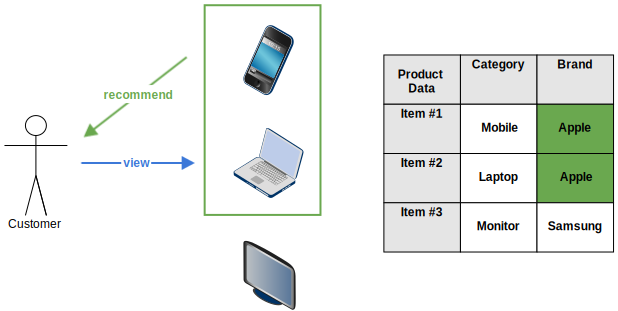
\includegraphics[width=0.7\textwidth,center]{intro/background/contentbased.pdf}
    \caption{Content-Based Filtering Diagram}
    \label{fig:intro-techniques-contentbased}
\end{figure}

Content-based recommendation methods compare item features to find similar items. Based on items the user has shown a preference for before -- such as \emph{rated} or \emph{purchased} -- other similar items are looked up based on features of this item. Figure \ref{fig:intro-techniques-contentbased} illustrates a customer who has rated an item positively. The recommender engine compares the rated item with other items, finds another item, which has the same brand and therefore recommends that item.

Demographic filtering is a specialisation of content-based filtering putting emphasis on user rather than item features. A very basic demographic filtering can be achieved by regular content-based recommender engines by sourcing user data as items. The content-based recommender engine, implemented as part of this project does not distinguish between users and items, thus is able to handle demographic queries as well.

\subsubsection{Hybrids}
\label{intro-bg-tech-hybrid}

Hybrid recommender engines make use of two or more individual recommender engines -- hereinafter referred to as components. This is in particular interesting as it enables hybrid engines to utilise different kind of filtering techniques at once. A possible motivation of using hybrid engines is to overcome weaknesses of one engine with another. However it is also possible to combine systems implementing the same technique but e.g. using different data sources.

There are many possible ways of combining techniques, which are outlined in the proposal. In this project, a \emph{weighted} hybrid recommender engine is implemented which combines the scores of its components using a linear formula. A score is a numerical preference rank attached to recommendations.

\section{Objectives}
\label{intro-objectives}

\subsection{Development of an Integration Framework}
\label{intro-objectives-framework}

\subsection{Development of Collaborative and Content-Based Recommender Engines}
\label{intro-objectives-engines}

\subsection{Integration into a Demo Application}
\label{intro-objectives-demo}

\subsection{Abstraction}
\label{intro-objectives-abstraction}

This objective aims a separation of a system into smaller, loose coupled components and suggests the following criteria:

\begin{description}
    \item[Complexity] Applications such as recommender engines tend to be complex. If not separated, every component adds to the overall complexity making change very difficult, time consuming and expensive. Any change requires knowledge, testing and probably modifications of the whole system.
    \item[Dependency] If a system needs to be modified or even replaced, tightly coupled components become a dependency leading to expensive and tiresome rework.
    \item[Encapsulation] Information hiding is the main motivation behind encapsulation. The more information and implementation is hidden, the looser the coupling becomes. The benefit is that internal changes do not affect other components at all as long as the interfaces remain the same.
    \item[Database Abstraction] Recommender engines with direct access to databases of integrating applications are problematic as these systems are affected by any change of these databases.
    \item[Reusability] Tightly coupled components are difficult to reuse. Reusability is the main driver for multi-purposefulness of this project.
\end{description}

\subsection{Ease of integration}
\label{intro-objectives-easeofintegration}

The complexity and cost of integration of new systems into existing applications is a major constraint for many projects. This objective covers the ease of integration of applications as well as new recommender techniques. The code footprint, interactions and data volumes of the communication interfaces are typical measures of complexity.

\subsection{Multi-Purpose \& Interoperability}
\label{intro-objectives-multipurpose}

A \emph{multi-purpose} recommender engine is able to cope with different data sources and techniques. Ideally this system is extendable for possible forthcoming, yet unknown requirements.

This multi-purposefulness can be also described in the interoperability between recommender engines. \citet{manouselis07} differentiate between three criteria:

\begin{description}
    \item[Interoperability of the recommendation queries] which allows the same query to be reused. This can be achieved by variable parameters in the query.
    \item[Interoperability of the user and the domain models] which allows the exchange of models and other data among different recommender engines.
    \item[Interoperability of the recommendation results] which empowers recommender engines to reuse the results. This is in particular useful for hybrid recommender engines.
\end{description}

\subsection{Technological Unbiasedness}

The proposal noted another objective to build a mechanism, which allows the integration of various recommender techniques to \emph{coexist} and \emph{cooperate}. \emph{Coexistence} refers to supporting various recommender techniques and solutions regardless of technology, language, storage technology and operating system. Furthermore, \emph{cooperation} emphasises the aforementioned interoperability between those recommenders.

\section{Structure of the Report}

\begin{description}
    \item[Chapter 2] illustrates the architecture and concepts of various systems of the project.
    \item[Chapter 3] goes into detail and describes the implementation, testing and technology choices.
    \item[Chapter 4] evaluates the project against the project objectives.
    \item[Chapter 5] reflects on the project outcome and possible future work.
    \item[Appendix A] contains the bibliographical references of the report.
    \item[Appendix B] offers user manuals of the various systems implemented.
    \item[Appendix C] lists the source code written for this project.
\end{description}